\chapter{Application of multi-device computation to a detailed city-scale surface-water flood simulation}
\label{chapter:ScaleEffects}

The domain decomposition methods provided in the last chapter allow simulations to be accelerated considerably when compared to traditional single-core CPU-bound software. This capability allows the spatial extent and resolution of simulations to be pushed beyond the realms previously considered, and as such creates new research questions surrounding the limits of data presently available, predictive capability of the models, and future data requirements.

This chapter considers a real-world pluvial flood event, by leveraging all of the data which could be obtained, and processing power available to the author at the time of writing.

\section{Flooding in Newcastle during June and August 2012}

\begin{figure*}[tpb]
	\centering
	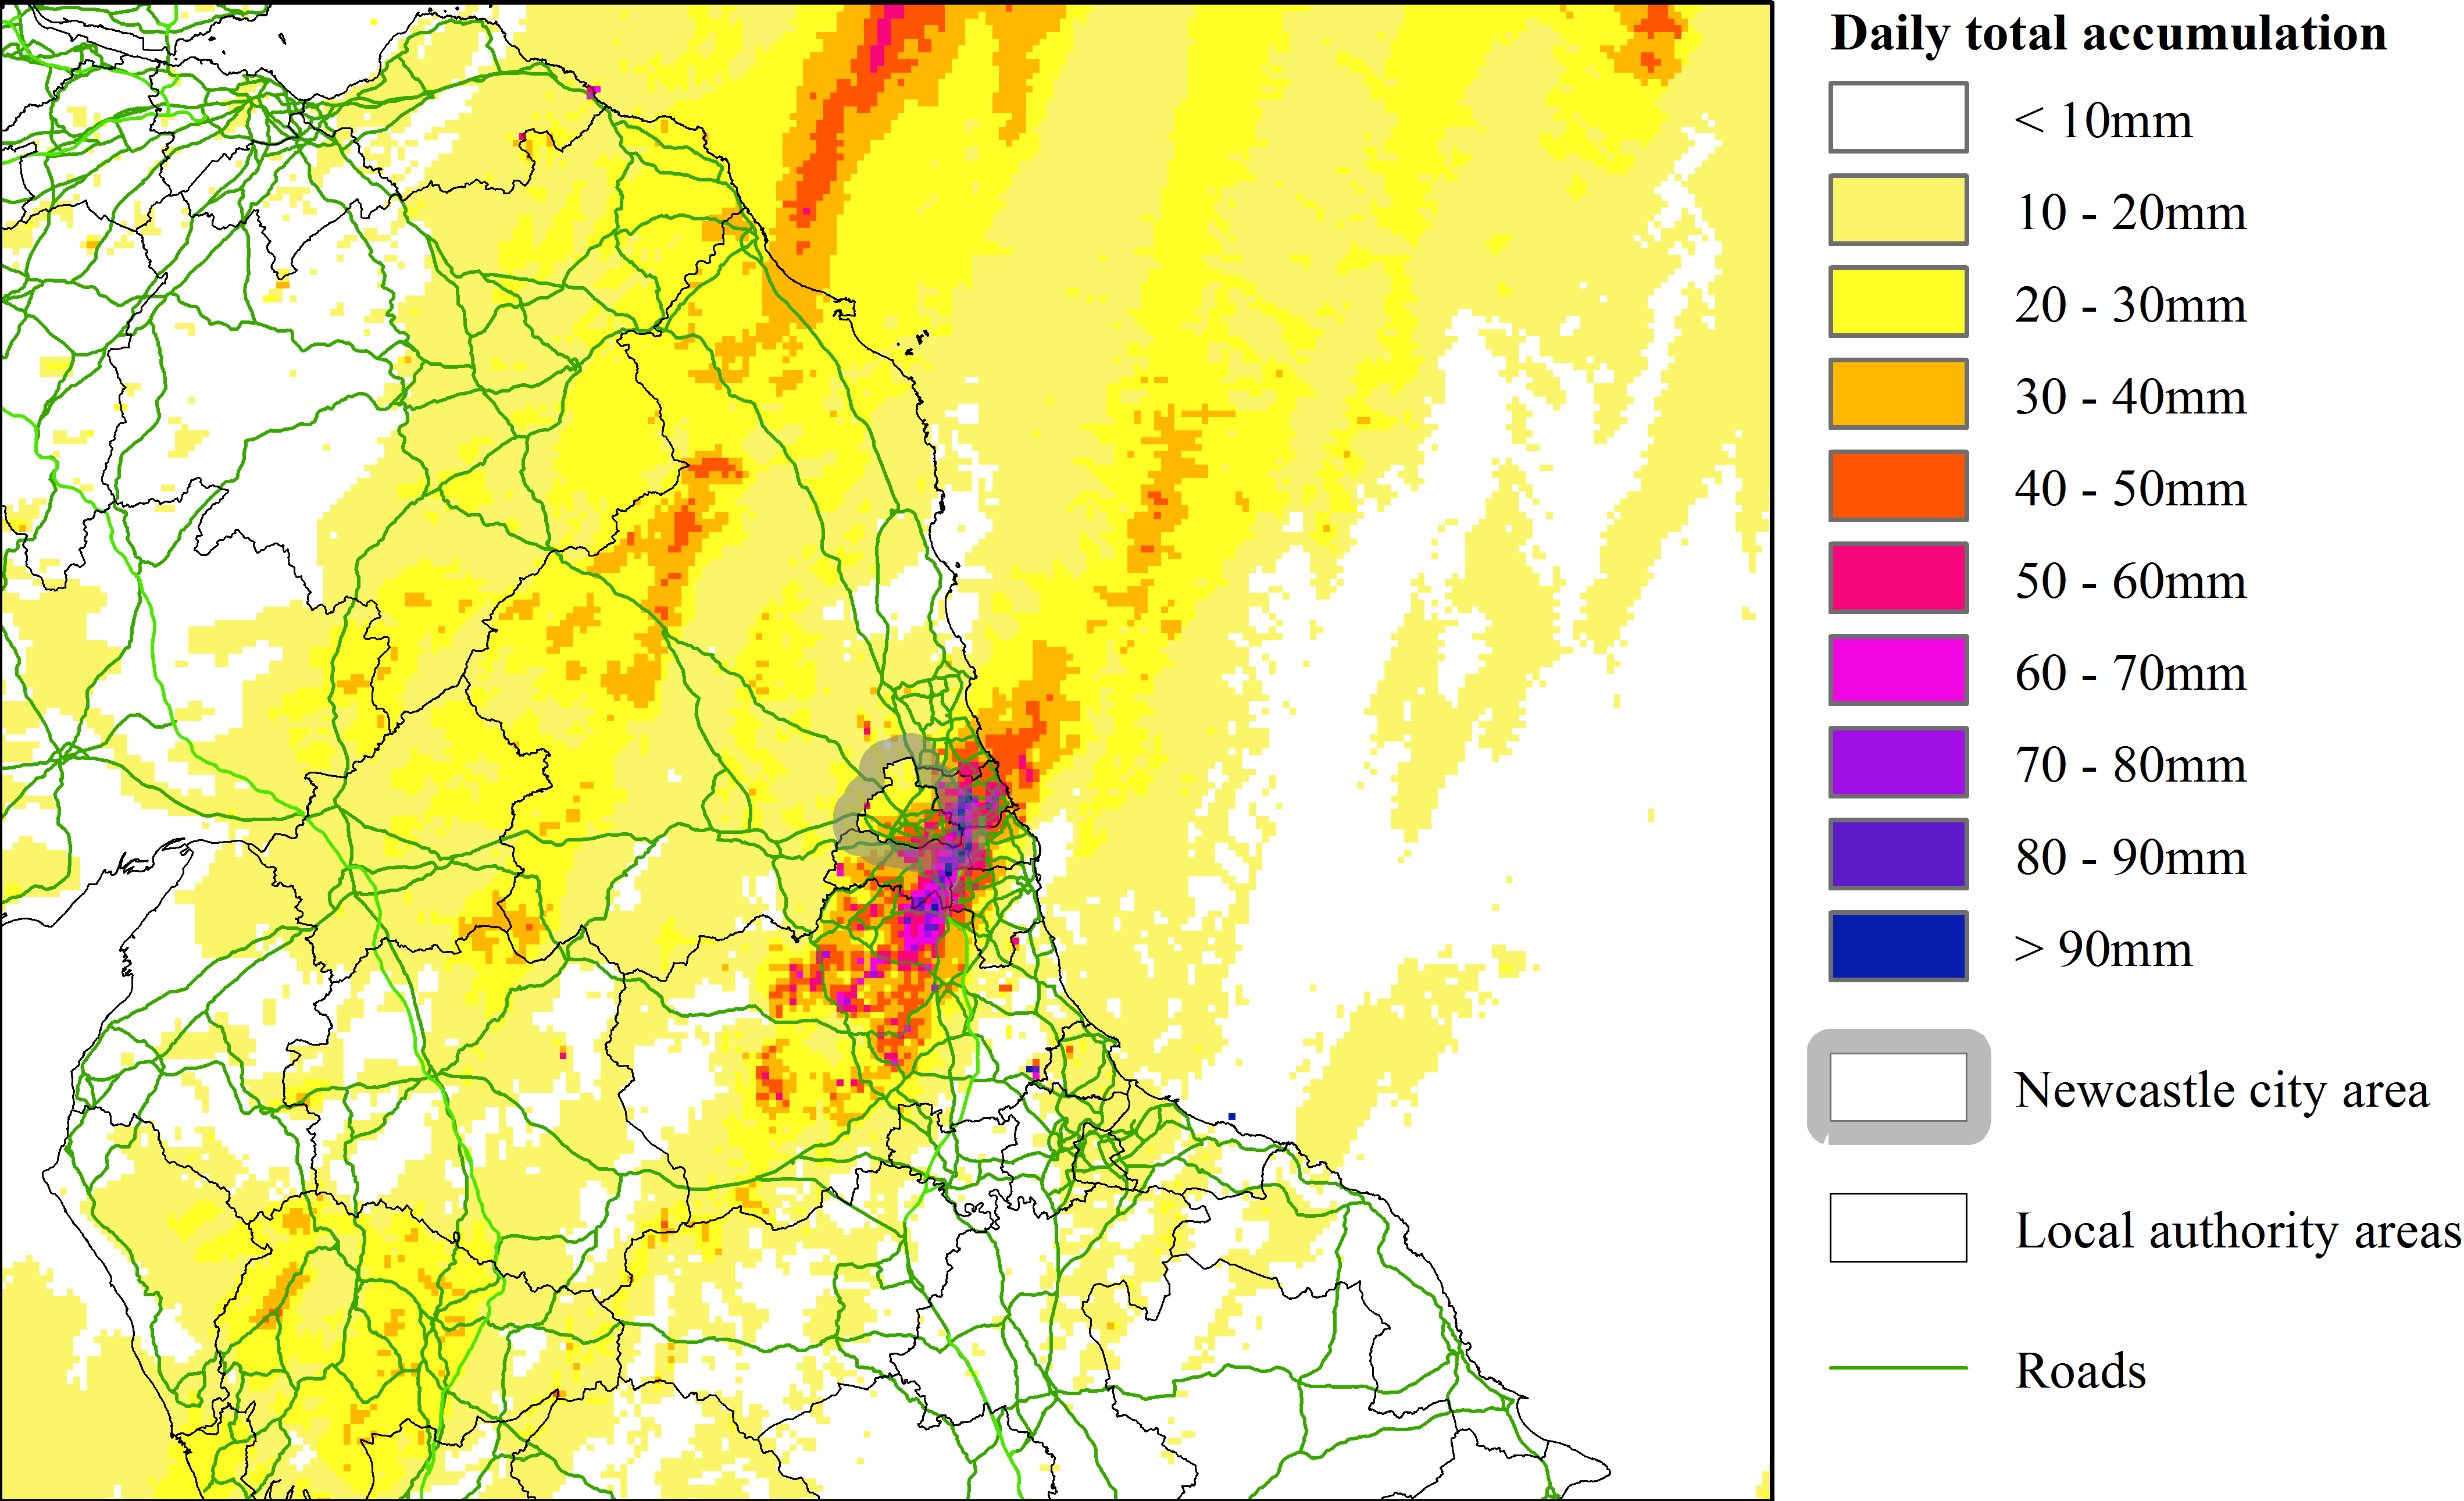
\includegraphics[width=1.0\textwidth]{newcastle-pluvial-figures/radar-rainfall-totals.png}
	\caption{Rainfall totals derived from rainfall radar for the flooding in Newcastle and the surrounding region, on 28 June 2012.}
	\label{Newcastle_Pluvial_RainTotal}
\end{figure*}

One of the most publicised floods in the UK during 2012 occurred in Tyne and Wear on 28th June 2012, during a month where many parts of the country were battered by short-duration heavy rainfall and thunderstorms over already saturated ground \citep{JBARiskManagement2012}. A supercell storm hit the city of Newcastle upon Tyne in North East England and the surrounding area at approximately 15:00, leaving the worst impacts to coincide with the peak evening commute. The effects of up to 50mm of rainfall during two hours were dramatic: Newcastle Central Station was flooded and the surrounding railway lines flooded or damaged by landslides; underground stations on the area's light rail network were flooded; grade-separated (i.e. overlapping infrastructure with different elevations) junctions connecting the city to all of the major arterial roads were flooded; and bus services were suspended in some areas. Many were stranded with no way to get home. More than 300 properties were flooded internally, and damage to highways alone in the Newcastle area was estimated at up to £8 million \citep{NewcastleCityCouncil2013}. Rainfall intensity varied greatly, both spatially and temporally across the city, but in some instances an intensity exceeding 200mm/hr was recorded for a short duration \citep{EnvironmentAgency2012a}.

The flooding manifested from a quasi-stationary convective storm, typified by thunder and a thick substantial layer of cloud, greatly reducing visibility and creating night-like conditions. The pattern was such that only a narrow band suffered the highest rainfall accumulations, whilst ten kilometres to the east or west received very little. The highest accumulations were believed to be slightly to the east of the city centre, as can be shown from the radar totals in Figure \ref{Newcastle_Pluvial_RainTotal}.

\section{Data sources and model generation}

Initially, two simulations have been carried out with a 2m resolution, one covering 36km$^{2}$ of Newcastle central area and another covering 400km$^{2}$ of Tyne and Wear, which respectively involve $~8$ million and $100$ million computational cells. The extent of the larger of these domains is shown in Figure \ref{Newcastle_Pluvial_DomainExtent}, along with the location of photos solicited from the public. Due to the flashy nature of the flood event, no organized field measurements are available for model validation, hence crowd-sourced data was relied upon; these were in the form of textual descriptions, photographs and videos submitted by the public.

\begin{figure*}[tpb]
	\centering
	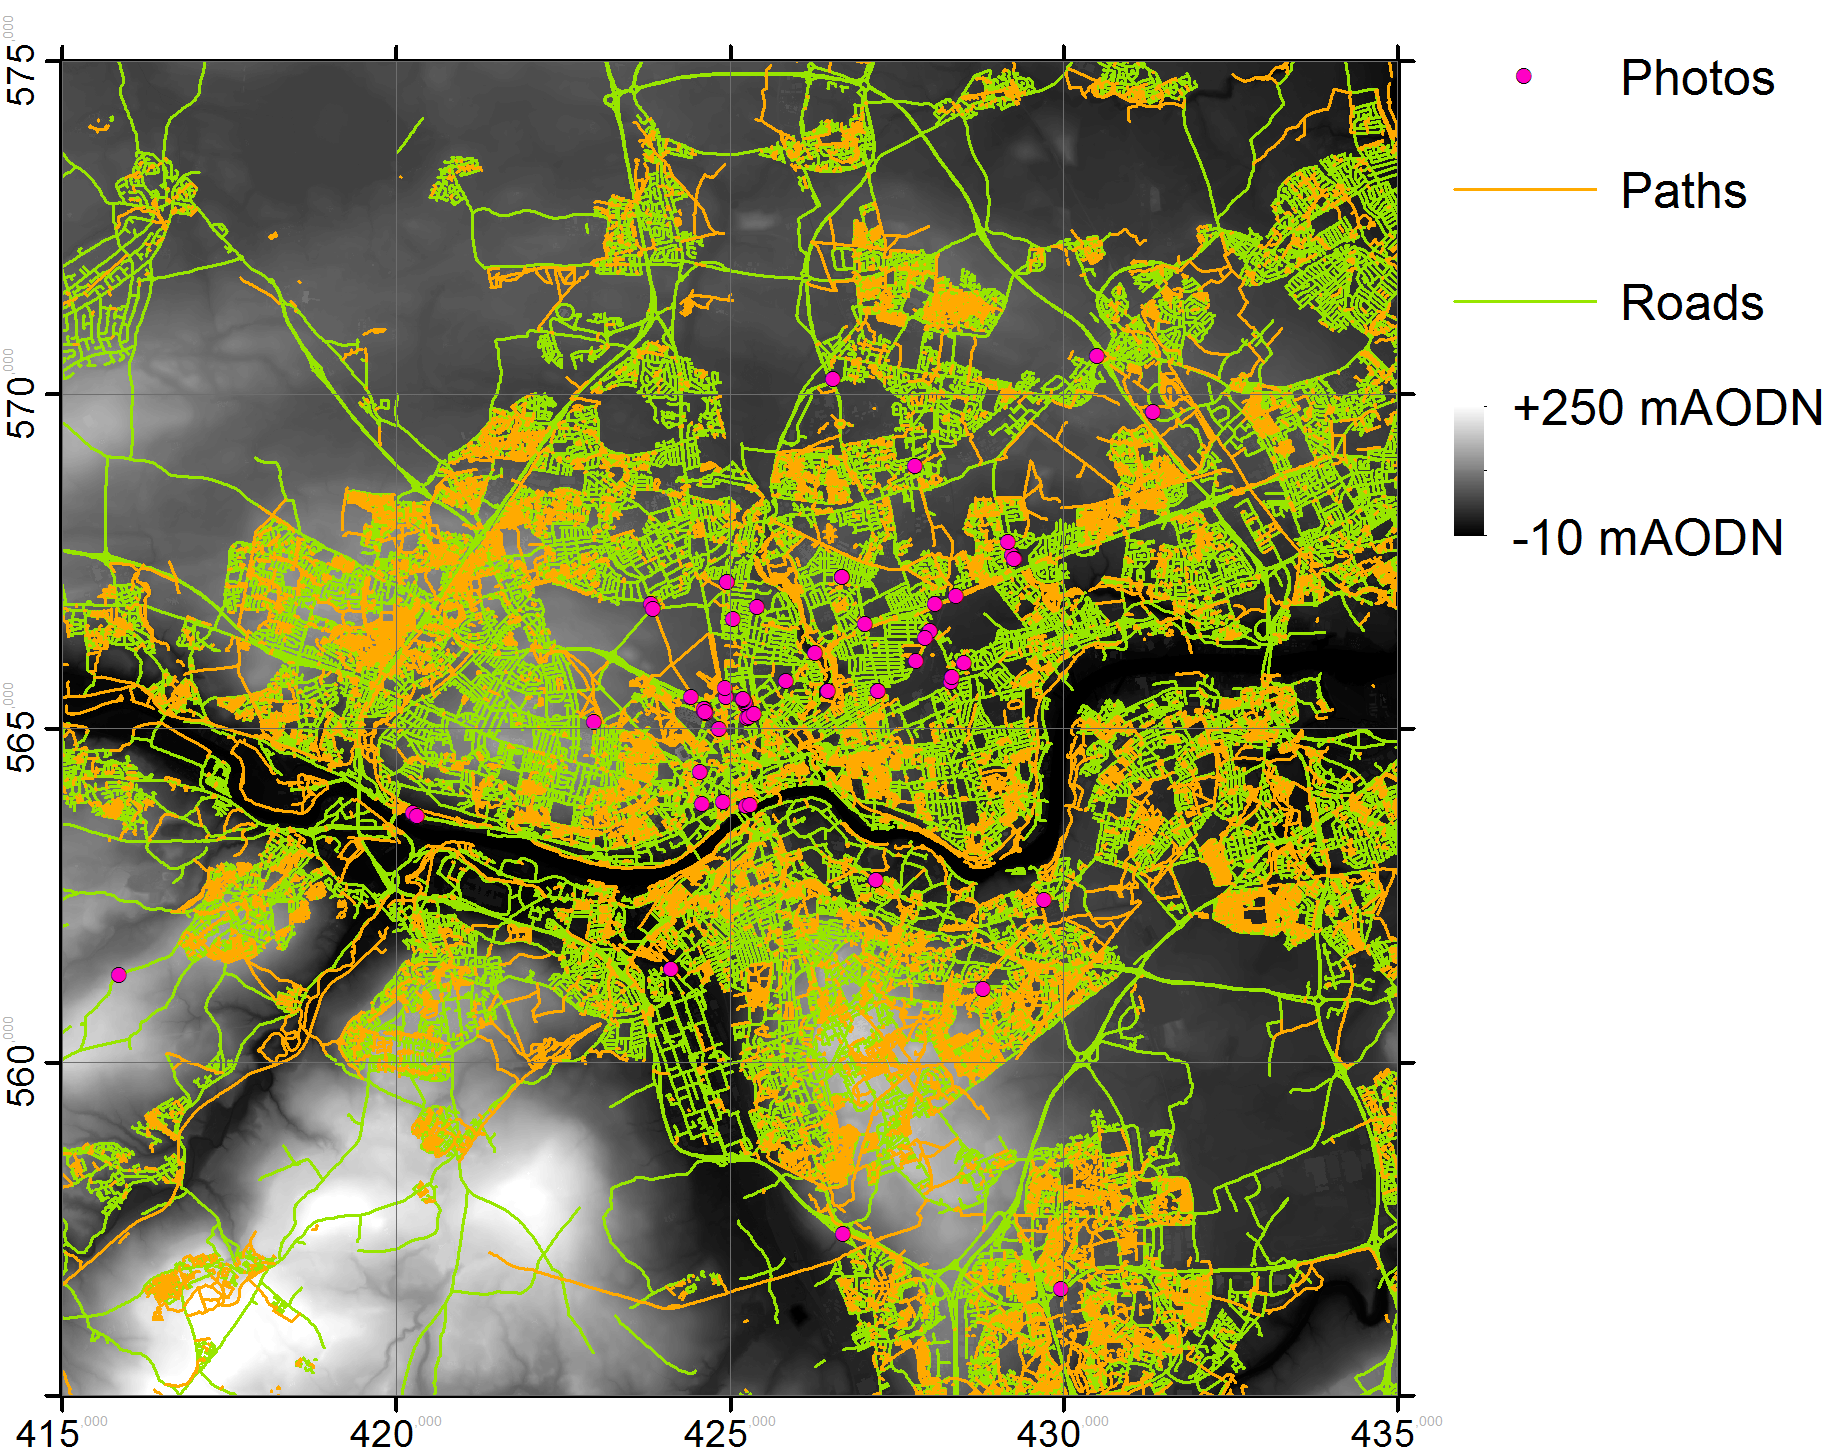
\includegraphics[width=1.0\textwidth]{newcastle-pluvial-figures/20km-domain-extent.png}
	\caption{Model extent for the 20 $\times$ 20km area around Tyne and Wear used to simulate flooding on 28 June 2012.}
	\label{Newcastle_Pluvial_DomainExtent}
\end{figure*}
\begin{sidewaysfigure}
	\centering
	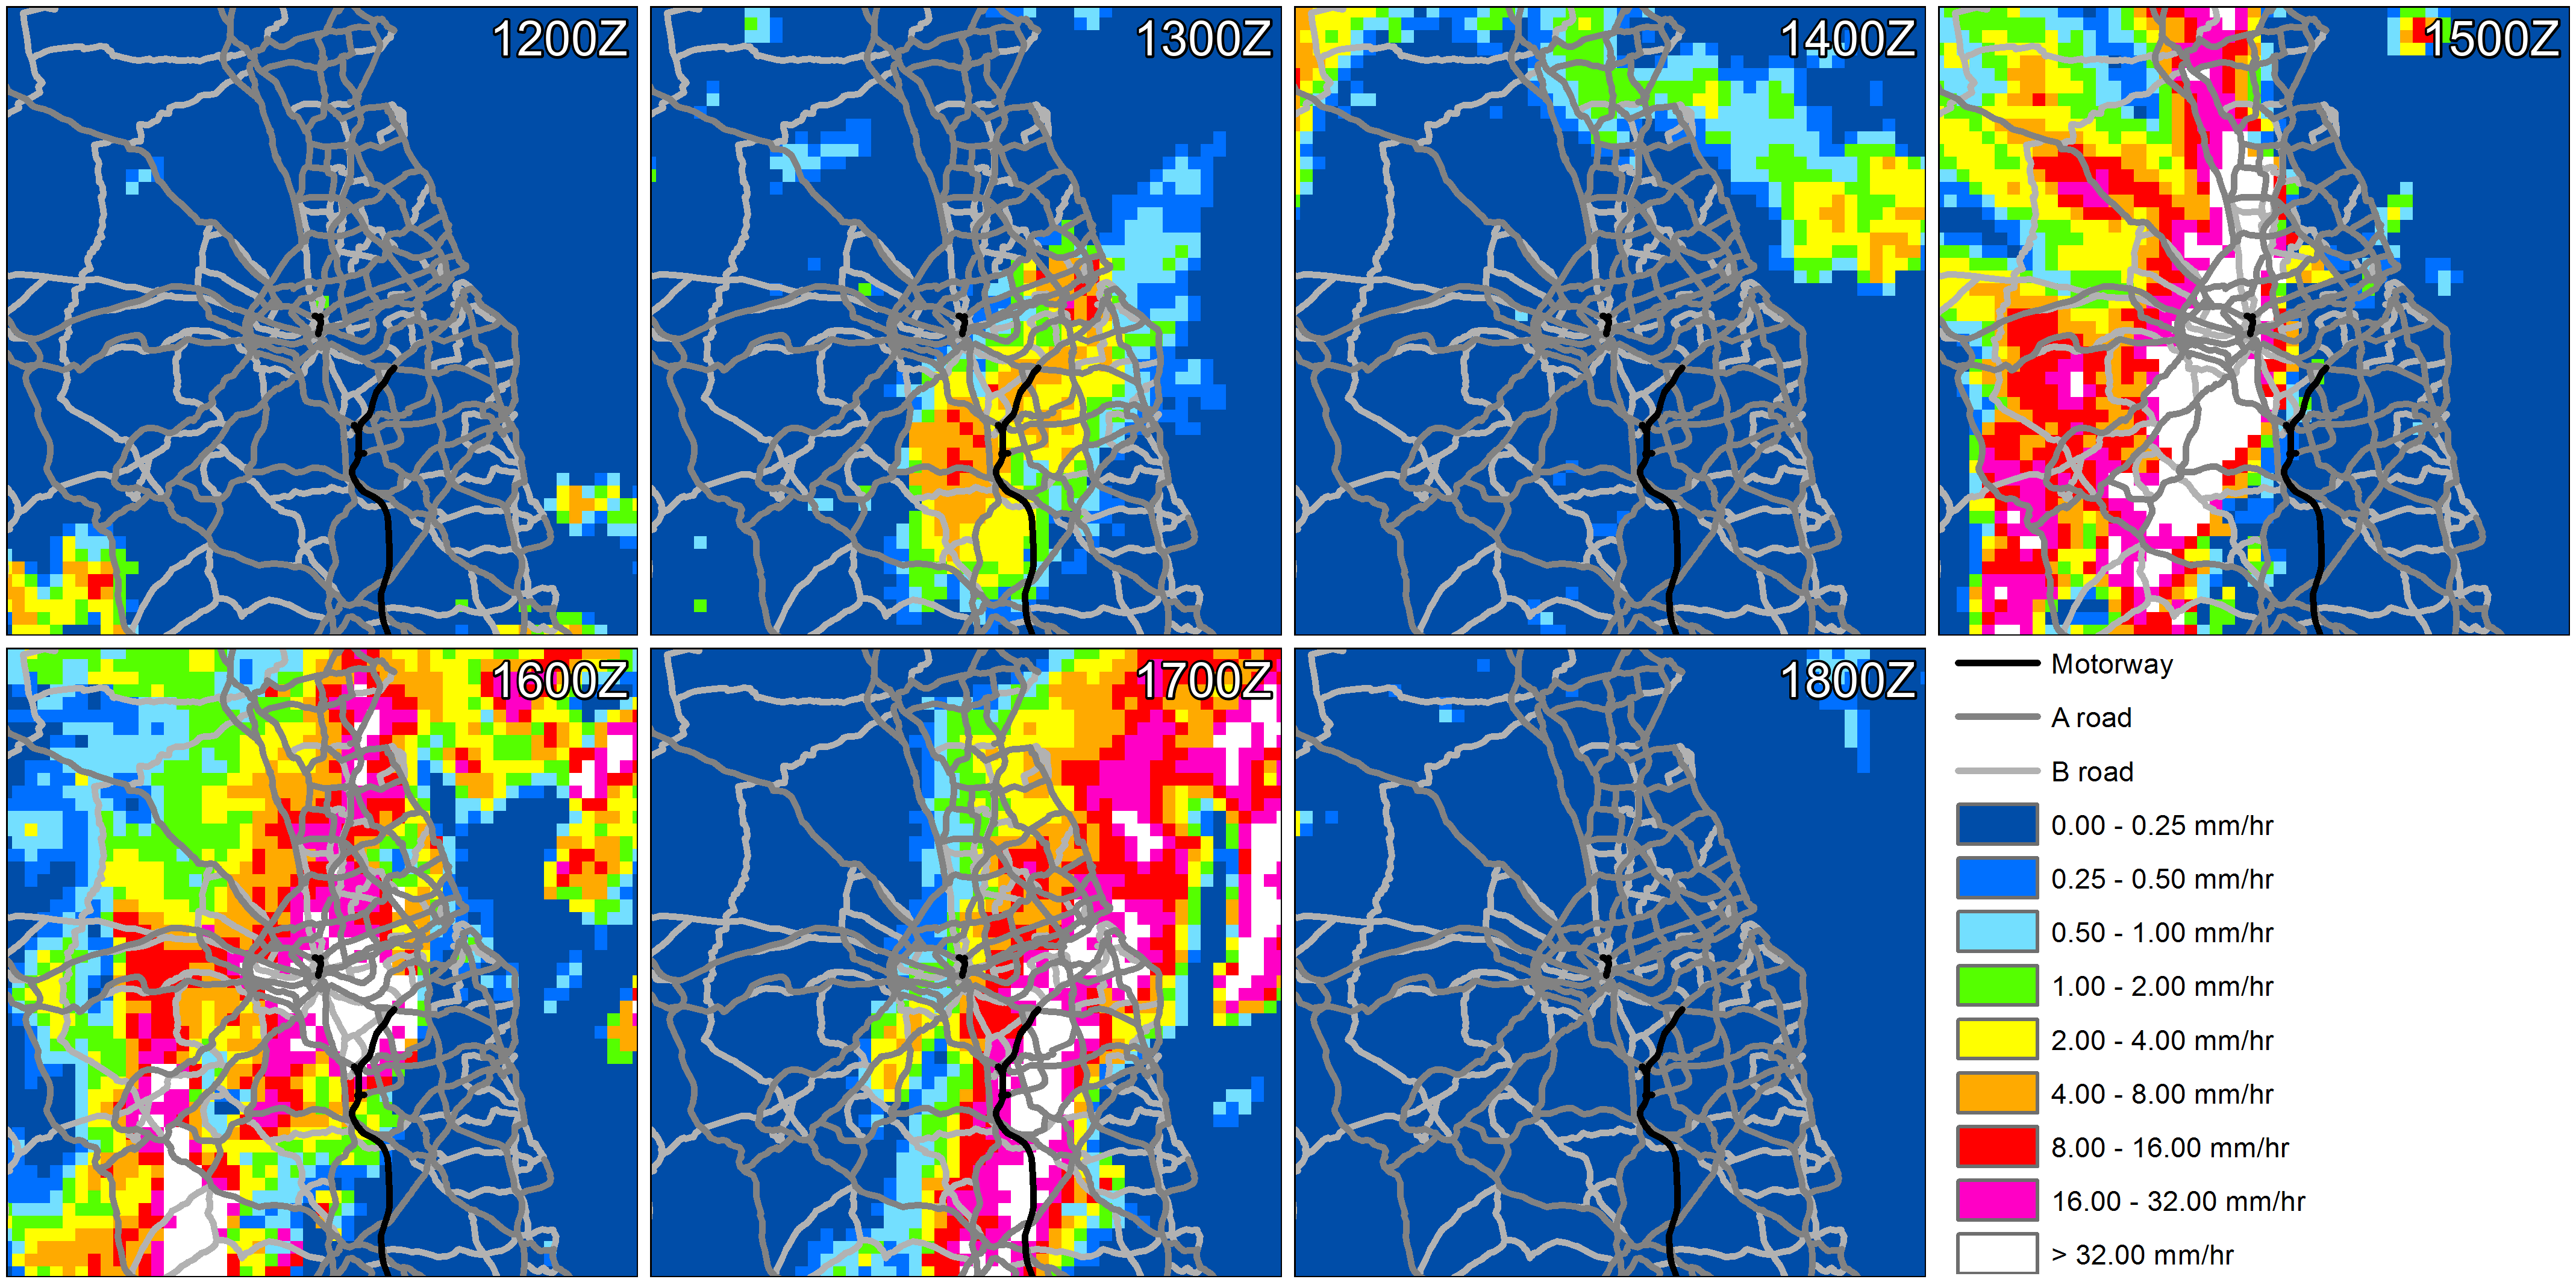
\includegraphics[width=1.0\textwidth]{newcastle-pluvial-figures/radar-rainfall-sequence.png}
	\caption{Rainfall radar timeseries centred on Newcastle upon Tyne, showing intensities for the 28 June 2012 event.}
	\label{Newcastle_Pluvial_Radar}
\end{sidewaysfigure}

Domain inputs used for all simulations were extracted from UK Met Office C-band rainfall radar (NIMROD) from 12:00 UTC to 18:00 on 28 June 2012, shown in Figure \ref{Newcastle_Pluvial_Radar}. Comparison of radar data against tipping bucket raingauges on the ground suggests good agreement. The Tyne and Wear model covers the full extent with highest rainfall totals, for the flood event considered as per rainfall radar. Specifically, this spans from $(415000, 555000)$ to $(435000, 575000)$ on the British National Grid (OSGB36). Bed elevations are in effect a digital elevation model, obtained by superimposing buildings from the first-pass return of an Environment Agency LiDAR survey atop a filtered terrain model, blended with OS Terrain 5 data where LiDAR coverage was lacking. This produces an elevation model where buildings are present, as important in determining the direction of flow, but vegetation which would provide minimal flow resistance (e.g. trees and bushes) are omitted. Buildings are not superimposed in the case of bridges and similar overhead structures, where a viable flow pathway is likely to exist beneath. Whilst imperfect insofar as there may be locations where flow could exist on two different levels within the same location, this is considered to be a practical compromise.

Generation of the elevation model was automated by processing OS MasterMap Topography Layer data to identify building outlines and overhead structures. A Manning coefficient of 0.2 is used across the whole domain; sensitivity testing suggested minimal effect on flood depths for this model. Cells which would ordinarily contain water, including ponds and rivers, were disabled from computation to allow the simulation to focus entirely on pluvial flooding processes. Domain decomposition is activated on the basis of synchronising timesteps.

The drainage network is not explicitly represented within the model, however as a substitute, a 12.5mm/hr drainage loss rate is applied to all cells, a figure which slightly exceeds the 10\% annual exceedance probability 2-hour duration event against which drainage infrastructure must be designed to withstand \citep{DMRB2016}, but is similar to the recommendations in Table 2 of BS EN 752:2008. This is also near-identical to the 12mm/hr "national average" rate adopted for England's surface water flood risk mapping \citep{EnvironmentAgency2013}.

Following the flood event, members of the public were invited to contribute photos and their respective locations for flooding through a dedicated website, which was advertised across the region using local television and radio. Social media activity from Twitter was also archived for analysis, which is examined in the next chapter. Areas worst affected were surveyed under instruction from the local council, with a questionnaire asking which areas of their property and the neighbouring infrastructure were affected. Briefing reports on the hydrology and its consequences were prepared by the Environment Agency and \citet{EnvironmentAgency2012a,NewcastleCityCouncil2013}.

\section{Results}

The software successfully provided results for the simulation, which are now considered against the evidence available for the actual extent of flooding, and discrepancies further analysed.

\subsection{Computational performance}

The simulations conducted were able to provide near real-time or faster prediction, for the six-hour period simulated, by leveraging multiple GPU devices. A sufficient number of identical processing devices was not available, hence two models of NVIDIA devices were mixed. These were four NVIDIA Tesla K40 and two K80 devices, where the latter is a single board which behaves as two discrete devices, so this manifests as eight devices in total. It is believed that further performance improvements could be achieved with the same software, if greater resources were made available, hence there is potential for these highly detailed simulations to be used in a predictive capacity in the future. The full performance details are given in Table \ref{PerformanceResults_MultiGPU_Newcastle}.

\begin{table*}[tbp]
	\small
	\centering
	\caption{Simulation run-times with different numbers of NVIDIA Tesla K40 and K80 devices, for the simulation of the Newcastle upon Tyne pluvial flood event on 28 June 2012, using different domain sizes}
	\label{PerformanceResults_MultiGPU_Newcastle}
	\begin{tabular}{p{0.15\linewidth}p{0.08\linewidth}p{0.15\linewidth}p{0.2\linewidth}p{0.15\linewidth}}
		\hline
		\multicolumn{5}{c}{\textbf{Performance results for simulations of the area surrounding Newcastle upon Tyne}} \\
		\hline
		Zone		 		& Area					& Resolution (cells)	& Devices						& Runtime (hh:mm:ss)	\\
		\hline
		Tyne and Wear		& $400 km^{2}$			& 2m (100,000,000)		& 4$\times$K40M 2$\times$K80	& 06:01:00				\\
		City centre			& $34 km^{2}$			& 2m (8,805,496)		& 4$\times$K40M 2$\times$K80	& 01:01:22				\\
		\hline
	\end{tabular}
\end{table*}

\subsection{Ability to reproduce large-scale flood features}

\begin{figure*}[tbp]
	\centering
	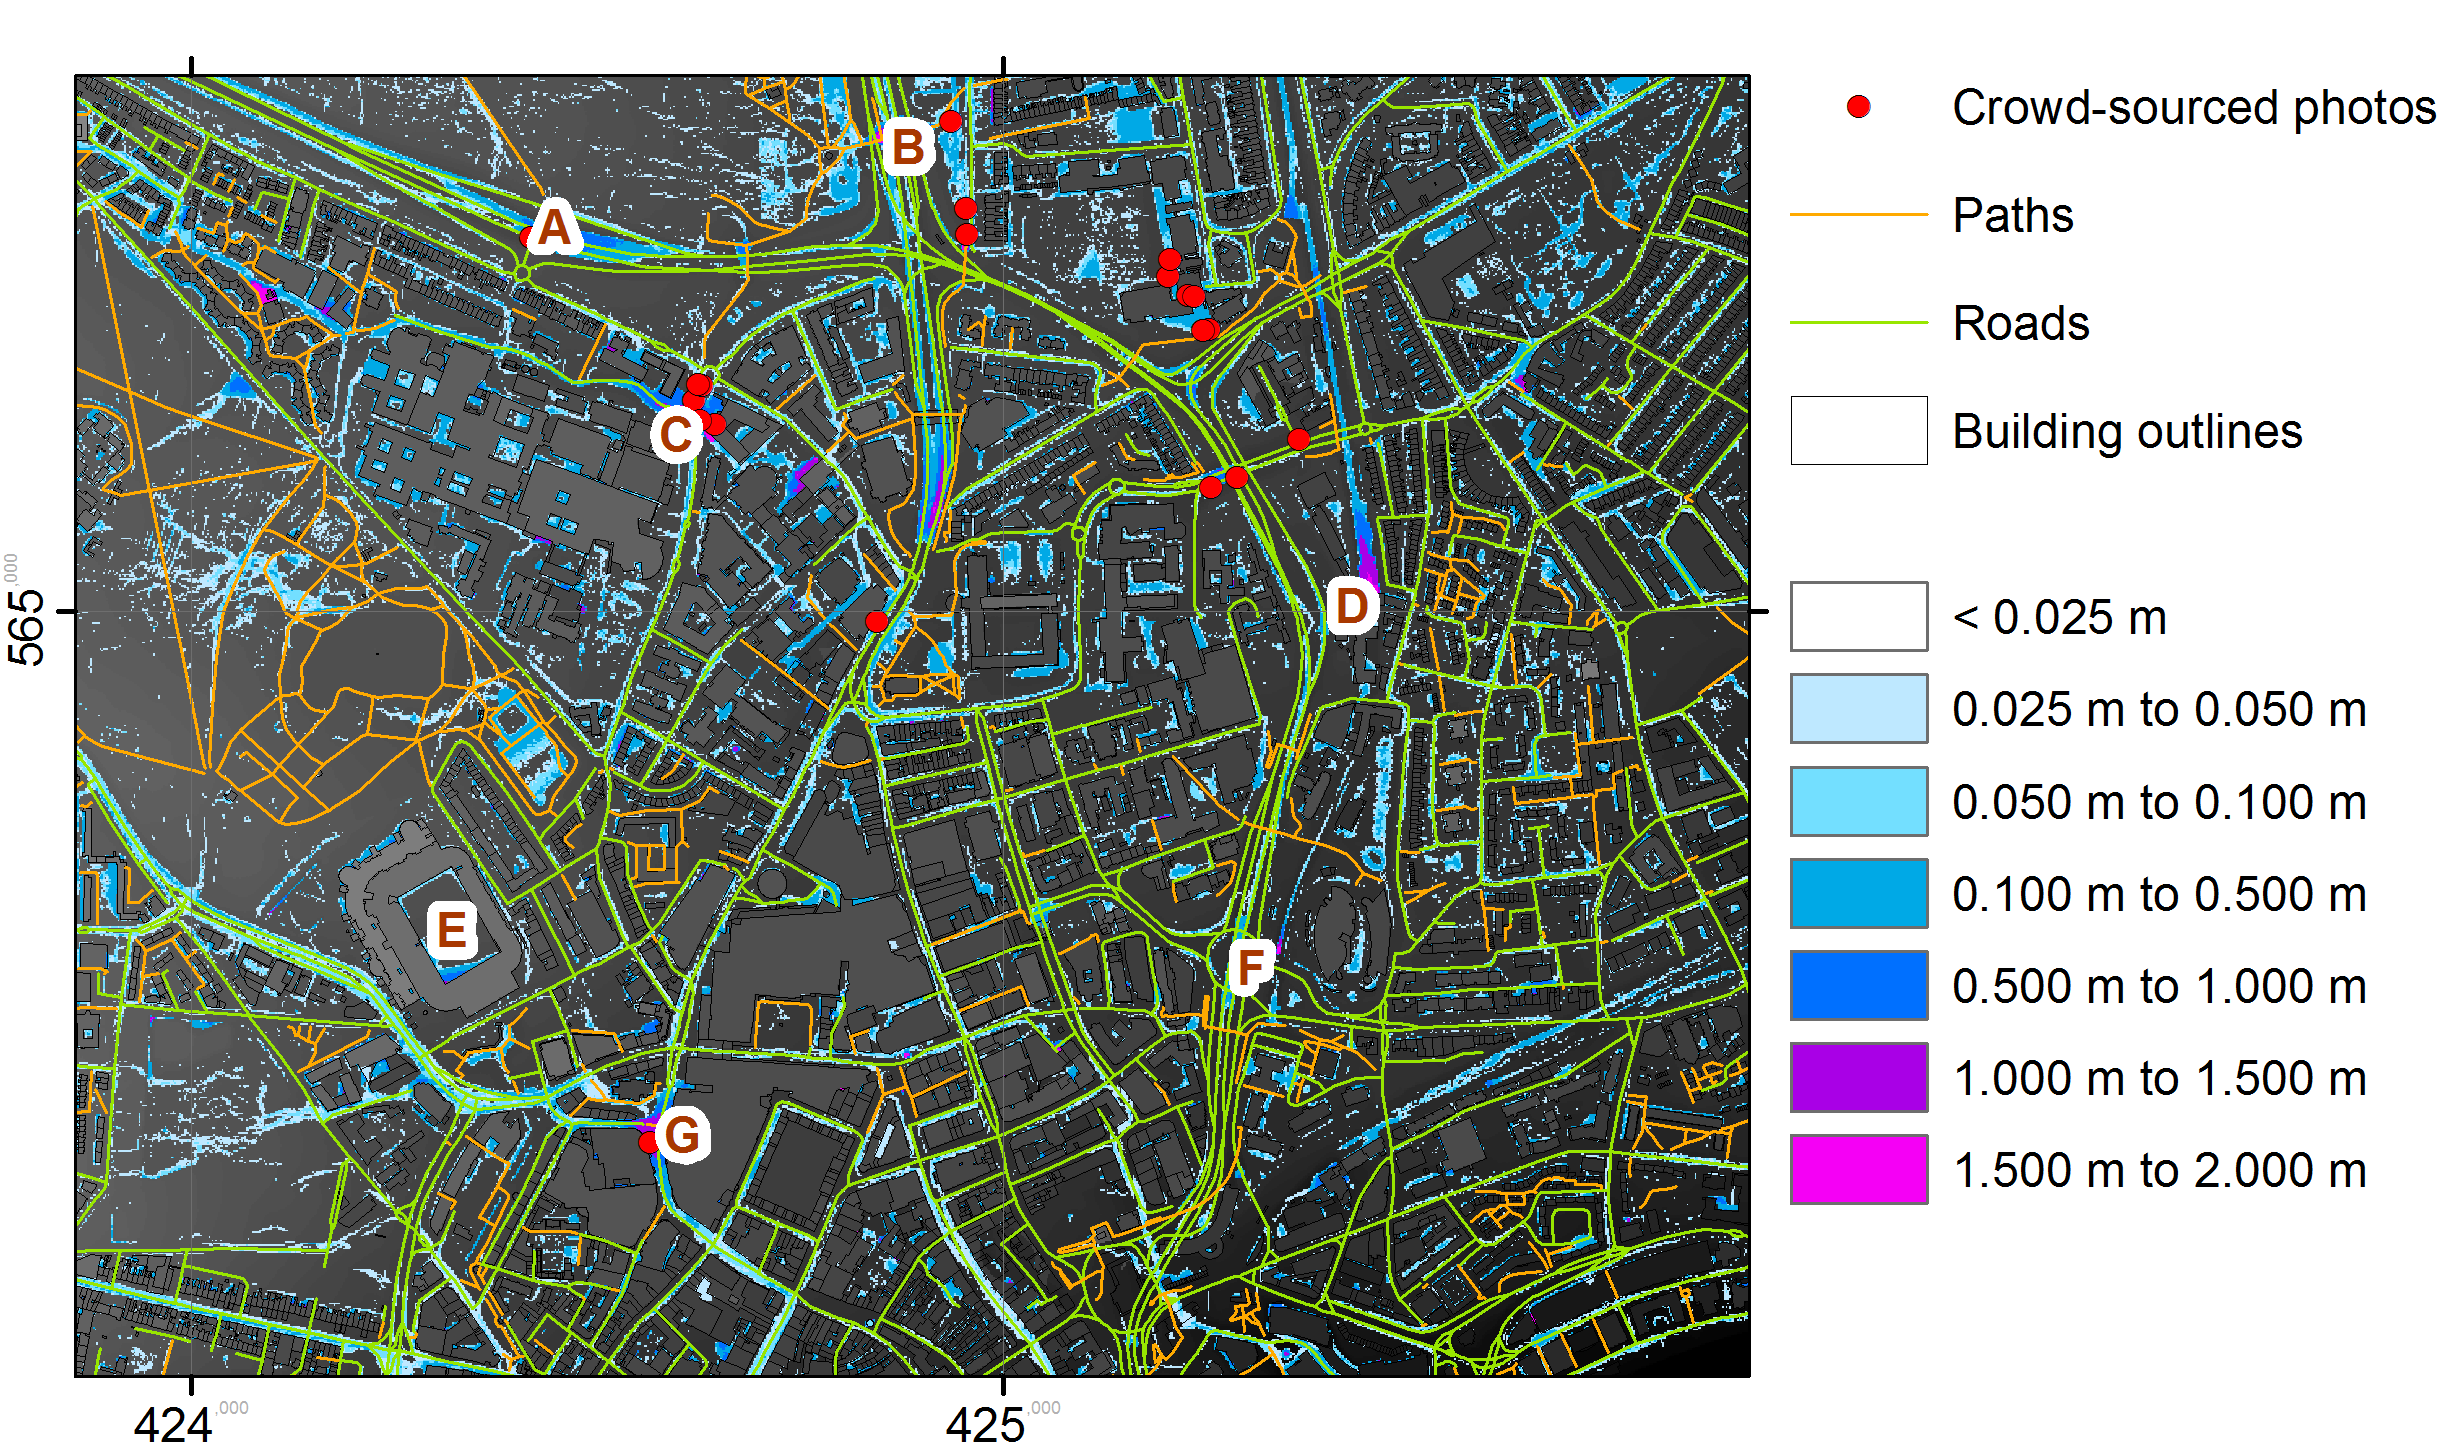
\includegraphics[width=1.0\textwidth]{newcastle-pluvial-figures/centre-depth-lettered.png}
	\caption{Extract of flood depths for a subsection of the simulation results, focusing on the centre of Newcastle upon Tyne.}
	\label{Newcastle_Centre_Depths}
\end{figure*}

The locations of a subset of photos received, alongside simulation results showing maximum depths, are shown in Figure \ref{Newcastle_Centre_Depths} for a small area of the city ($\approx$ 2 $\times$ 2km). It is clear there is strong agreement between the locations of the crowd-sourced photos and flooding. On the A167(M) Central Motorway, at points A and F it can be seen that dips in the road for intersections have suffered from serious flooding, which is an unfortunate consequence of the transport infrastructure design in Newcastle, and reinforces that some settlements are more exposed to the risk of pluvial flooding. Some of the longest overland flow pathways converge at point C on the Newcastle University campus, and G near The Gate entertainment complex, and these are clearly visible as some of the highest depths. Points E and D highlight some of the limitations of the approach, with the football pitch at E seeing exaggerated flooding because infiltration and drainage is inadequately represented, and a large pool appearing at D where in fact the railway line goes underground, but topographic data obtained did not reflect this. Point B represents a pedestrian passageway under a major road, which is accurately represented and was known to flood, however the road above is not represented and was also flooded. As a whole, the simulation results provide an accurate representation of the flooding which occurred in June 2012, albeit with scope for improvements by manual intervention in some places where the LiDAR does not fully capture the complex reality of topography.

\begin{figure*}[tbp]
	\centering
	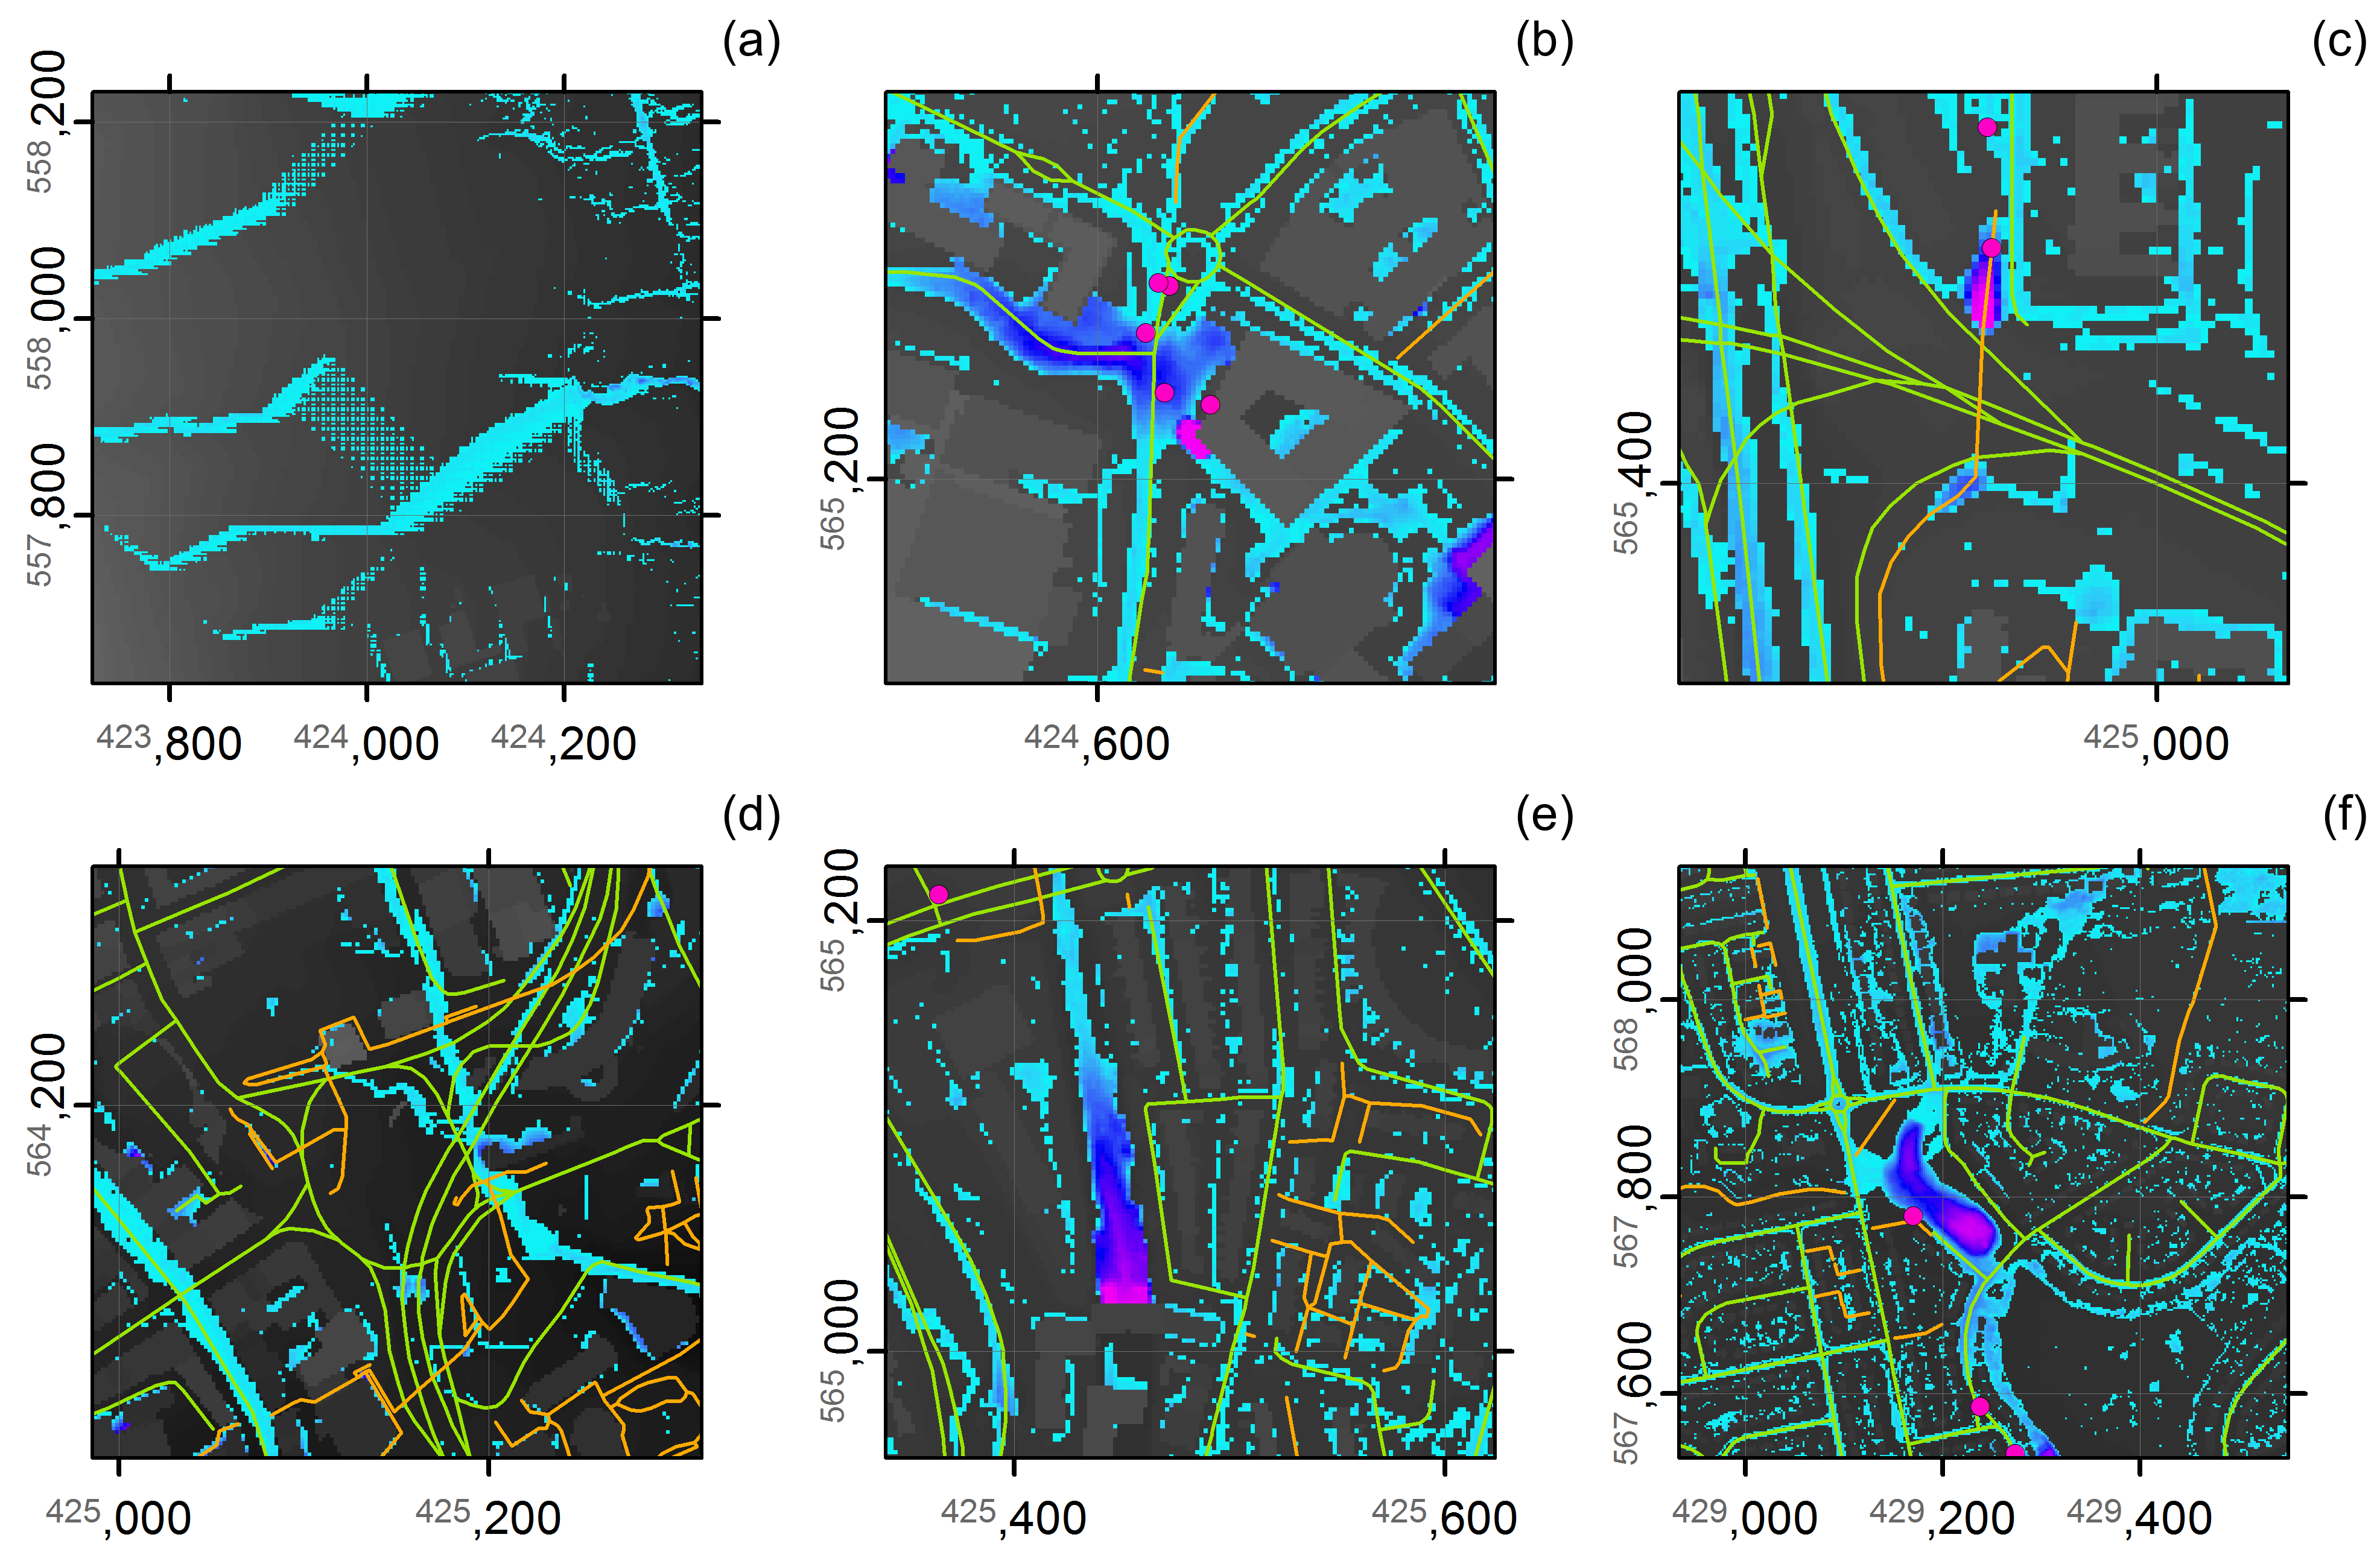
\includegraphics[width=1.0\textwidth]{newcastle-pluvial-figures/focal-areas.png}
	\caption{Sample areas of interest from the model results, showing (a) checkerboard effect with coarse DTM source data, (b) exaggerated depths above a large drainage culvert, (c) flooding predicted around underpasses, (d) complex network of underpasses and road tunnels, (e) railway tunnel not represented properly, and (f) sacrificial land area.}
	\label{Newcastle_Focal_Areas}
\end{figure*}

Examining the results for the model domain as a whole, some specific areas of interest have been extracted and are shown in Figure \ref{Newcastle_Focal_Areas}. Whilst resampled 5m DTM data provides a basis for ensuring flow connectivity in areas where 2m LiDAR coverage was lacking, the results in the 5m areas are not satisfactory. The checkerboarding effect shown in (a) is a consequence of the inferior numerical resolution of the 5m DTM data and resampling algorithm. A blur-like filter would be necessary to smooth these features, but this could also reduce the severity of genuine gradients. Increased LiDAR coverage remains essential to improving our understanding of surface water flood risk. The flooding shown in (b) is exaggerated slightly; this area is underlain by a large culverted watercourse now used as a sewer, which is not represented by the drainage assumptions made uniformly across the domain. It is important to note that even with more information, accurately predicting the capacity of this long-culverted watercourse would prove difficult. Flooding in pedestrian underpasses is a known issue in Newcastle upon Tyne; while they are not necessarily captured by the single-level DEM used by the model, in many cases the entrances to the underpasses are sunk and therefore capture risk, such as shown in (c) but not as well represented for a more complex network of underpasses, tunnels and roads shown in (d). Accurate data for the railway network in the UK, including the alignment of tunnels, was not available and hence the backwater shown in (e) is an erroneous artefact of a railway tunnel under a number of buildings. The area shown in (f) did flood, but not to the extent shown; this is a basin used as sacrificial land (designed as flood storage during extreme conditions), with a children's playground for use during normal conditions. The uniform drainage assumptions have underestimated the capacity of the soil infiltration in this area.

There are further considerations not examined in detail here, such as the need for greater ubiquity of LiDAR coverage outside of urban areas, thereby encompassing their upstream catchments, and the issues surrounding our limited knowledge of long-culverted watercourses and ageing drainage network, or antecedent conditions affecting infiltration capacity. Nonetheless the model results are a good match against crowd-sourced information from an event on 28 June 2012, despite notable areas where improvements could be made.

\subsection{Ability to reproduce small-scale flood features, and sensitivity to grid resolution}

To fully consider the impacts of grid resolution, further simulations were prepared, focusing on small areas of interest, Kensington Terrace. The area of the university campus has been comprehensively surveyed, including the position of drainage infrastructure such as grates. Large puddles (more than 2m diameter) are known to form on this road during and following periods of prolonged rainfall. The building heights are explicitly represented by the topographic grid, hence water runs from the pitched roofs to the nearby cells on the ground. The same event is simulated, and the results obtained using 1m, 2m, and 4m grids are shown in Figure \ref{Newcastle_Pluvial_CampusContours}.

The 4m simulation is clearly inferior, because the detail of the road grading is not captured at this resolution. The 2m simulation correctly predicts a long slender puddle down the side of the road, which frequently occurs in practice, while the 1m simulation exaggerates the depth of a single puddle towards the south of the domain. While far from conclusive, analysis of this area suggests 1m LiDAR data may be failing to capture the broader topography, in which artefacts are not removed by the averaging process at coarser resolutions. The road infrastructure is graded to channel water towards drains, and only the 2m simulation is showing this effect, where the conglomeration of drains in the south of the domain is coincident with the majority of the water.

The theory is tested by selecting a larger area of the city, a suburban area encompassing parts of Byker, Walker and Walkergate. Simulations were conducted from 1m to 32m, increasing exponentially. The results were then compared at the property level, against individual addresses for which questionnaire results were obtained. It must be acknowledged that there are obvious discrepancies in the questionnaire results, such as properties which reported no flooding whilst every single neighbour did, potentially borne of concern over future ability to obtain insurance, absence from the property during the event, or property-level protection features. The gardens and yards are assumed to represent the area without buildings, within the land parcel. The questionnaire refers to areas of road or pavement outside the property, hence GIS tools were used to prepare polygons which aligned to the property boundary for this purpose. No specific topographic data is shown herein, to protect the privacy of those who responded. 

\begin{figure*}[tpb]
	\centering
	\includegraphics[width=0.8\textwidth]{newcastle-pluvial-figures/campus-contours-resolutions.png}
	\caption{Comparison of results on part of the Newcastle University campus at different grid resolutions.}
	\label{Newcastle_Pluvial_CampusContours}
\end{figure*}
\begin{figure*}[p]
	\centering
	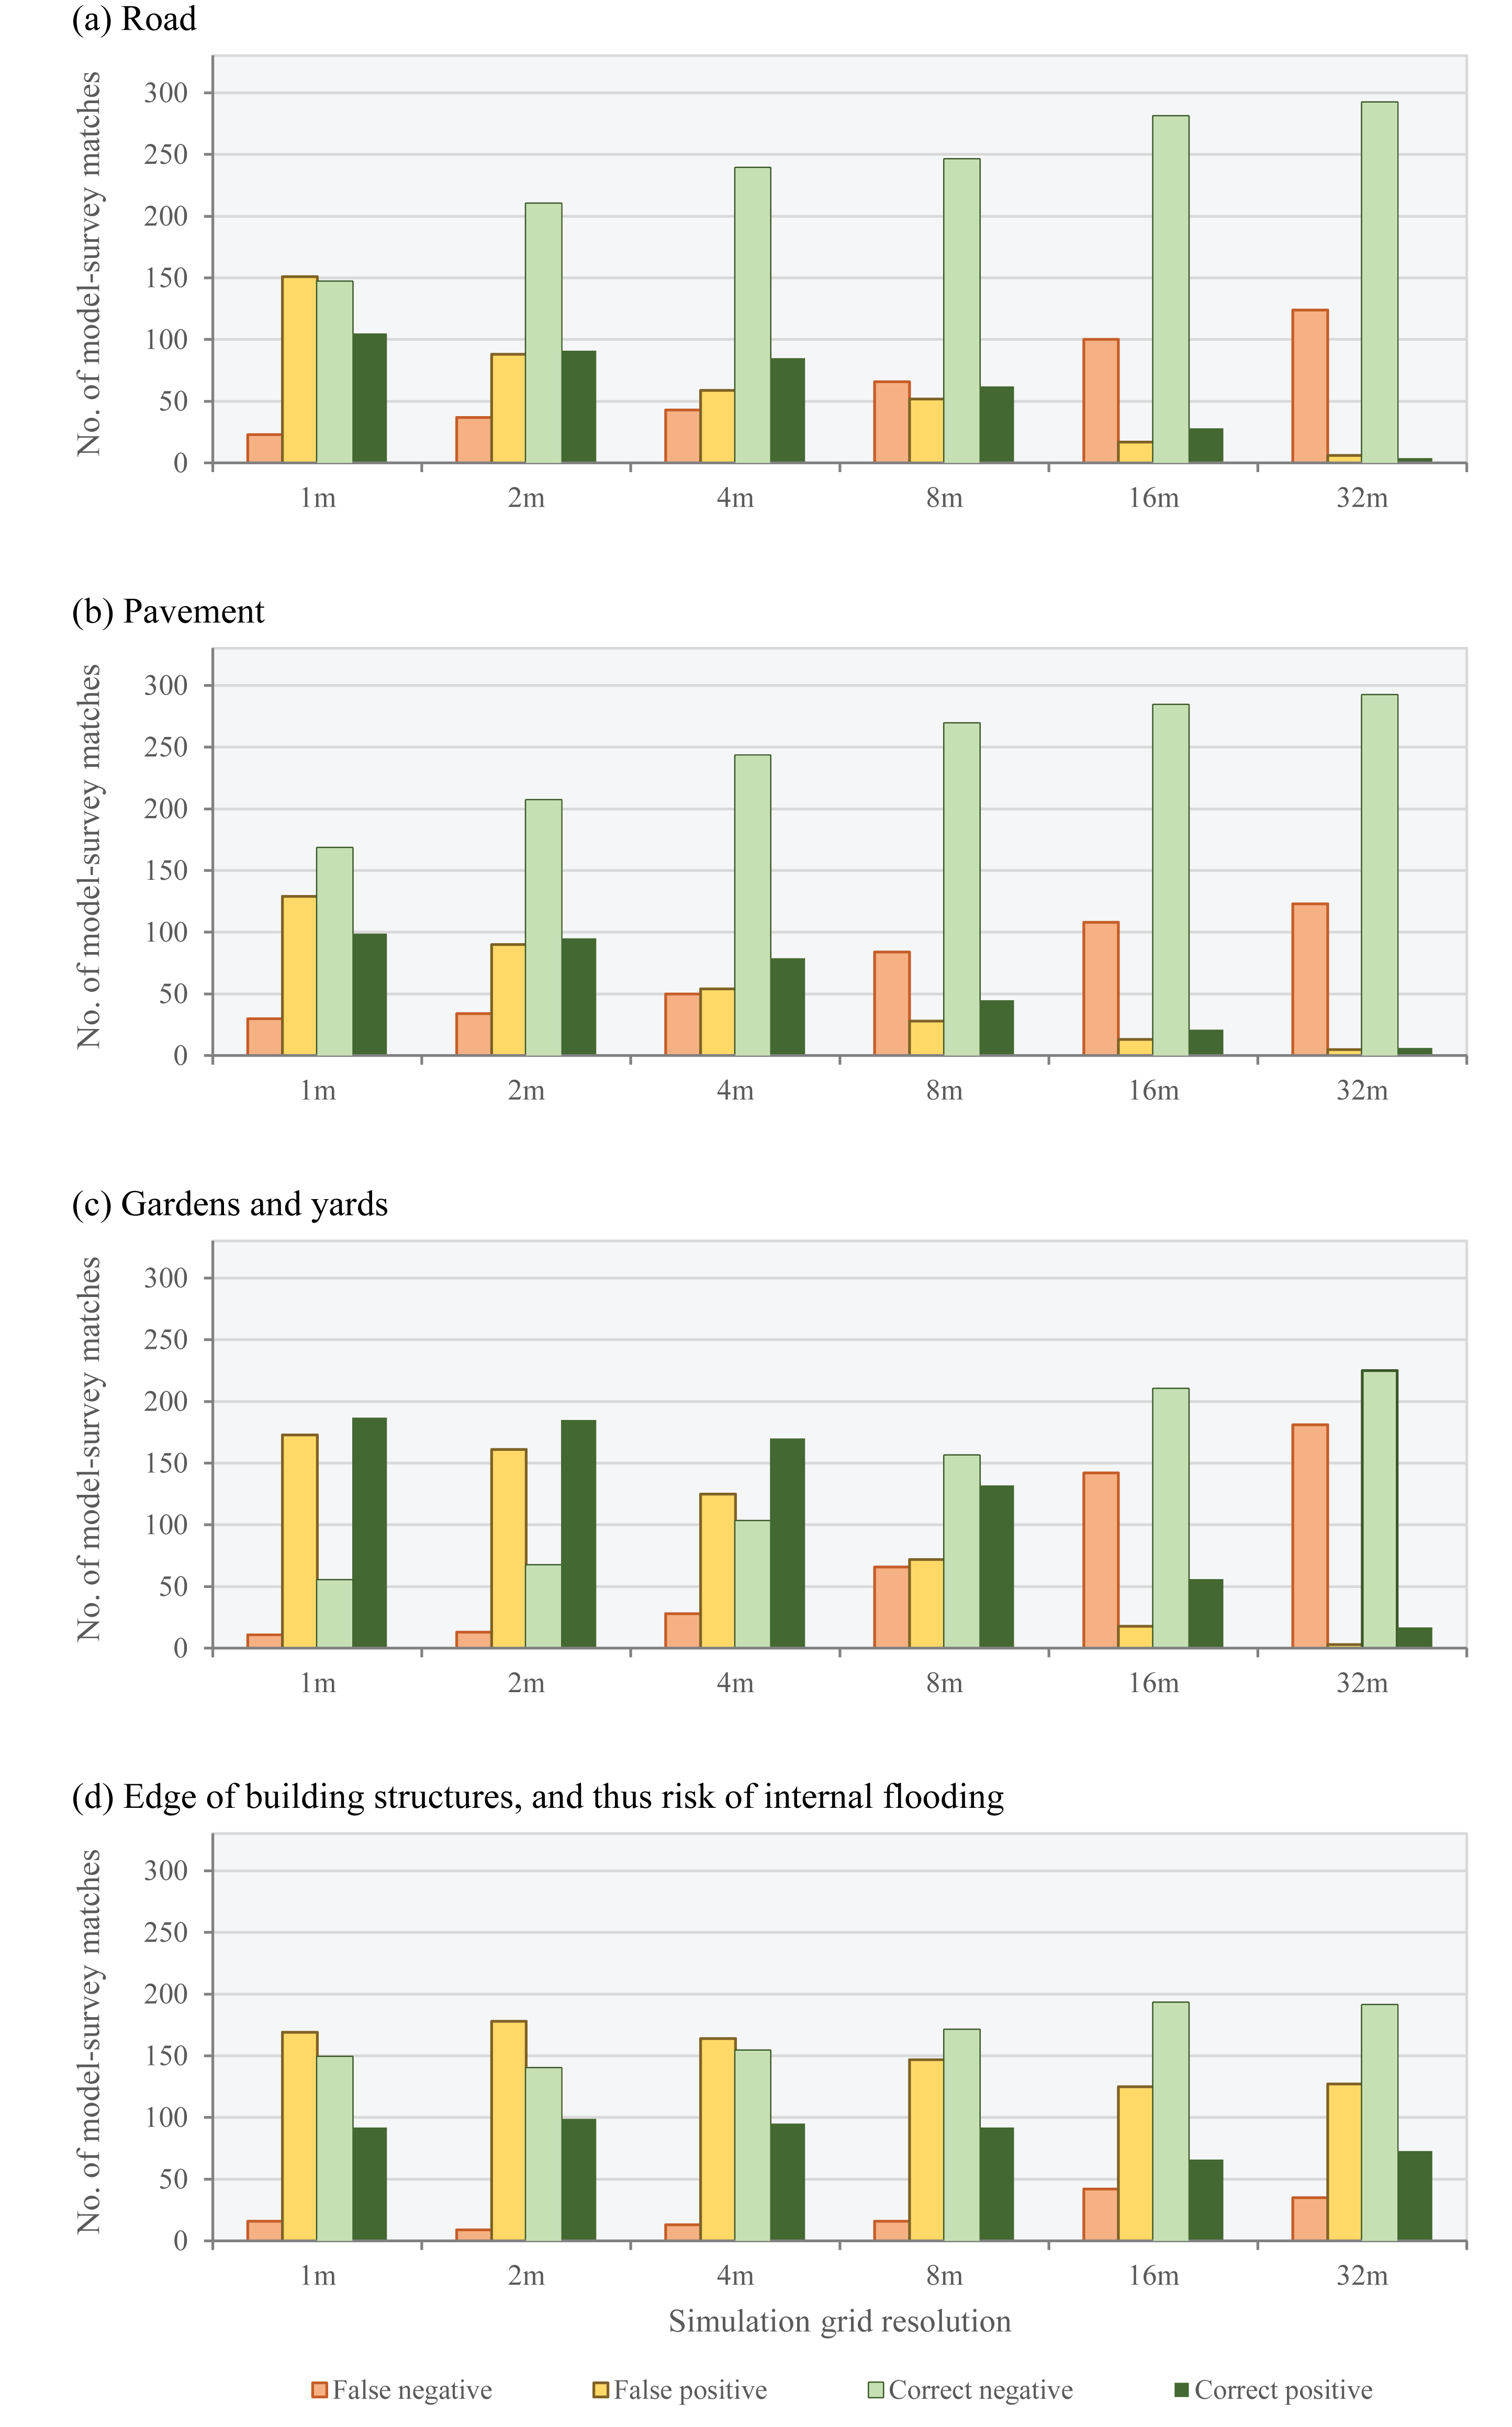
\includegraphics[width=0.85\textwidth]{newcastle-pluvial-figures/survey-matches.png}
	\caption{Comparison of result positive and negative results against survey data from residents for a suburban area of Newcastle.}
	\label{Newcastle_Pluvial_ResidentSurveyStats}
\end{figure*}

Statistics were derived for each of the zones around a respondent's property, classifying each against the simulation results for maximum depth, as false or correct, and negative or positive. The results are shown in Figure \ref{Newcastle_Pluvial_ResidentSurveyStats}.

In all cases, the 2m simulation provides a higher number of correct results when compared to 1m. Simulations at resolutions coarser than 4m perform extremely poorly, especially for road flooding, presumed to be because the road camber and pavements are not captured, and the water is displaced incorrectly; surface water flood risk assessments thus require simulations of 4m or better, which is a concern for areas not yet covered by LiDAR, where coarser datasets are used at present.

Prediction of flooding in gardens and yards provides the highest degree of confidence. Roads and pavements exhibit a high number of false positive results, further suggesting that the microtopography of the infrastructure is not captured in the data. There is also a question surrounding whether people would consider moving water (even if relatively deep) along a road, to constitute flooding. As expected, determining whether the interior of a building will flood remains the most difficult, because many factors affect this (e.g. the presence of airbricks, the installation of flood prevention measures, the elevation of the entrance to the property).

\section{Conclusions}

This chapter presented a simulation for a city-scale urban flood event induced by intense rainfall, reproduced at a very high resolution using domain decomposition. The largest simulation conducted herein was performed in the same length of time as the event under simulation, and there is scope for further acceleration with greater hardware resources. This simulation would not be feasible without leveraging heterogeneous computing and domain decomposition.

\begin{itemize}
	\item Computational performance itself should not be considered a limiting factor in hydraulic modelling, as software capable of leveraging heterogeneous and large distributed computer systems becomes increasingly widespread. 
	\item There is evidence that coarse resolution data used for surface water flood risk assessments in areas without LiDAR coverage is insufficient, and may provide extremely poor predictions.
	\item Determining whether the interior of a property is likely to flood remains difficult, and should not be considered as simple as whether water is neighbouring the structure.
	\item Artefacts within high resolution LiDAR data are believed to cause erroneous results in some simulations, especially with a resolution of 1m; obtaining higher resolution LiDAR data will alleviate this to a large extent as the artefacts can be smoothed during spatial averaging to a lower resolution.
	\item Improved representation of flooding in dense urban areas will benefit from grade-separation of flow pathways, thereby addressing areas in which tunnels flood in addition to the road surface above.
	\item Failure to represent the drainage network detracts from the accuracy of results in some areas, and exaggerates flow depths, while neglecting potential surcharging of the system elsewhere.
\end{itemize}

Comparing this pluvial flood event to the fluvial event in Carlisle, the validation data available is of inferior quality. The flashy nature of convective storms means traditional methods of data collection, such as surveying water and wrack marks, are not practical. Convective storms are also more difficult to accurately simulate, as rainfall intensities are highly variable and may not be contiguous, hence accurate and high resolution rainfall data is preferable. In the next chapter, the potential of social media is considered as an additional data source, with the same event used to evaluate its potential.